\section{Results and Discussion}

\subsection{Functional Verification}

The first result is categorical: every scenario behaved exactly as predicted by theory. Across 375 total trials, all 275 trials in theoretically valid scenarios produced the correct AES key and successfully decrypted the ciphertext, while all 100 trials in theoretically invalid scenarios failed during robust reconstruction. No case produced a false positive decryption.

This outcome directly matches the two central recovery rules:
\begin{itemize}
\item If there are no corrupted shares, recovery succeeds whenever at least $t$ shares are available.
\item If up to $e$ shares are corrupted, recovery succeeds only when $m \geq t + 2e$.
\end{itemize}

The corrupted-share scenarios are especially important because they distinguish the proposed method from ordinary threshold interpolation. For example, the $(t,n,m,e)=(3,5,5,1)$ scenario succeeded in all trials, whereas the $(3,5,4,1)$ scenario failed in all trials because the available redundancy was one share short of the theoretical bound.

\subsection{Failure Behavior}

The invalid scenarios failed for structural rather than incidental reasons. In all runs with $m<t$, the decoder had too few constraints to identify the degree-$(t-1)$ polynomial. In all runs with $m<t+2e$, the system lacked the redundancy needed to both identify the corrupted positions and reconstruct the correct polynomial. The implementation therefore raised decoding failure instead of returning a candidate key. This behavior is desirable because a key-recovery mechanism should fail conservatively when the mathematical recovery conditions are not satisfied.

The absence of false positives is particularly important in the corrupted-share setting. A naive reconstruction procedure that interpolates directly on all submitted points can produce a syntactically valid field element even when one or more shares are wrong. In contrast, the robust decoder in this study couples polynomial consistency checks with AES-GCM verification, so the recovery pipeline accepts only secrets that are algebraically and cryptographically consistent with the original instance.

\subsection{Timing Behavior}

The timing results show two consistent patterns. First, recovery is faster when the number of available shares is close to the minimum threshold, because the decoder solves a smaller linear system. Second, recovery time increases as either the threshold or the correctable error budget grows. This is visible when comparing the mean recovery times in Table~\ref{tab:scenarios}: the smallest successful configuration, minimum valid recovery with $(3,5,3,0)$, required only 0.0736 ms on average, while the largest successful no-error configuration, $(5,10,10,0)$, required 0.6451 ms.

The error-correction overhead is present but modest at the tested scale. For threshold $t=4$, moving from a normal full-share recovery $(4,7,7,0)$ to a two-error correction setting $(4,8,8,2)$ increased mean recovery time from 0.2937 ms to 0.4009 ms. Likewise, for threshold $t=5$, correcting two corrupted shares with nine available shares required 0.4787 ms on average. These values remain well below one millisecond, indicating that the algebraic overhead of robust reconstruction is practical for key-recovery workloads.

The failure cases in Fig.~\ref{fig:timing} also have a useful performance interpretation. Their measured latency is close to zero not because recovery becomes cheaper in a meaningful operational sense, but because the decoder terminates early once the share set is recognized as algebraically insufficient. This means that the additional redundancy required for robust recovery mainly affects the successful path, while invalid configurations are rejected with minimal extra computation.

\begin{figure}[H]
\centering
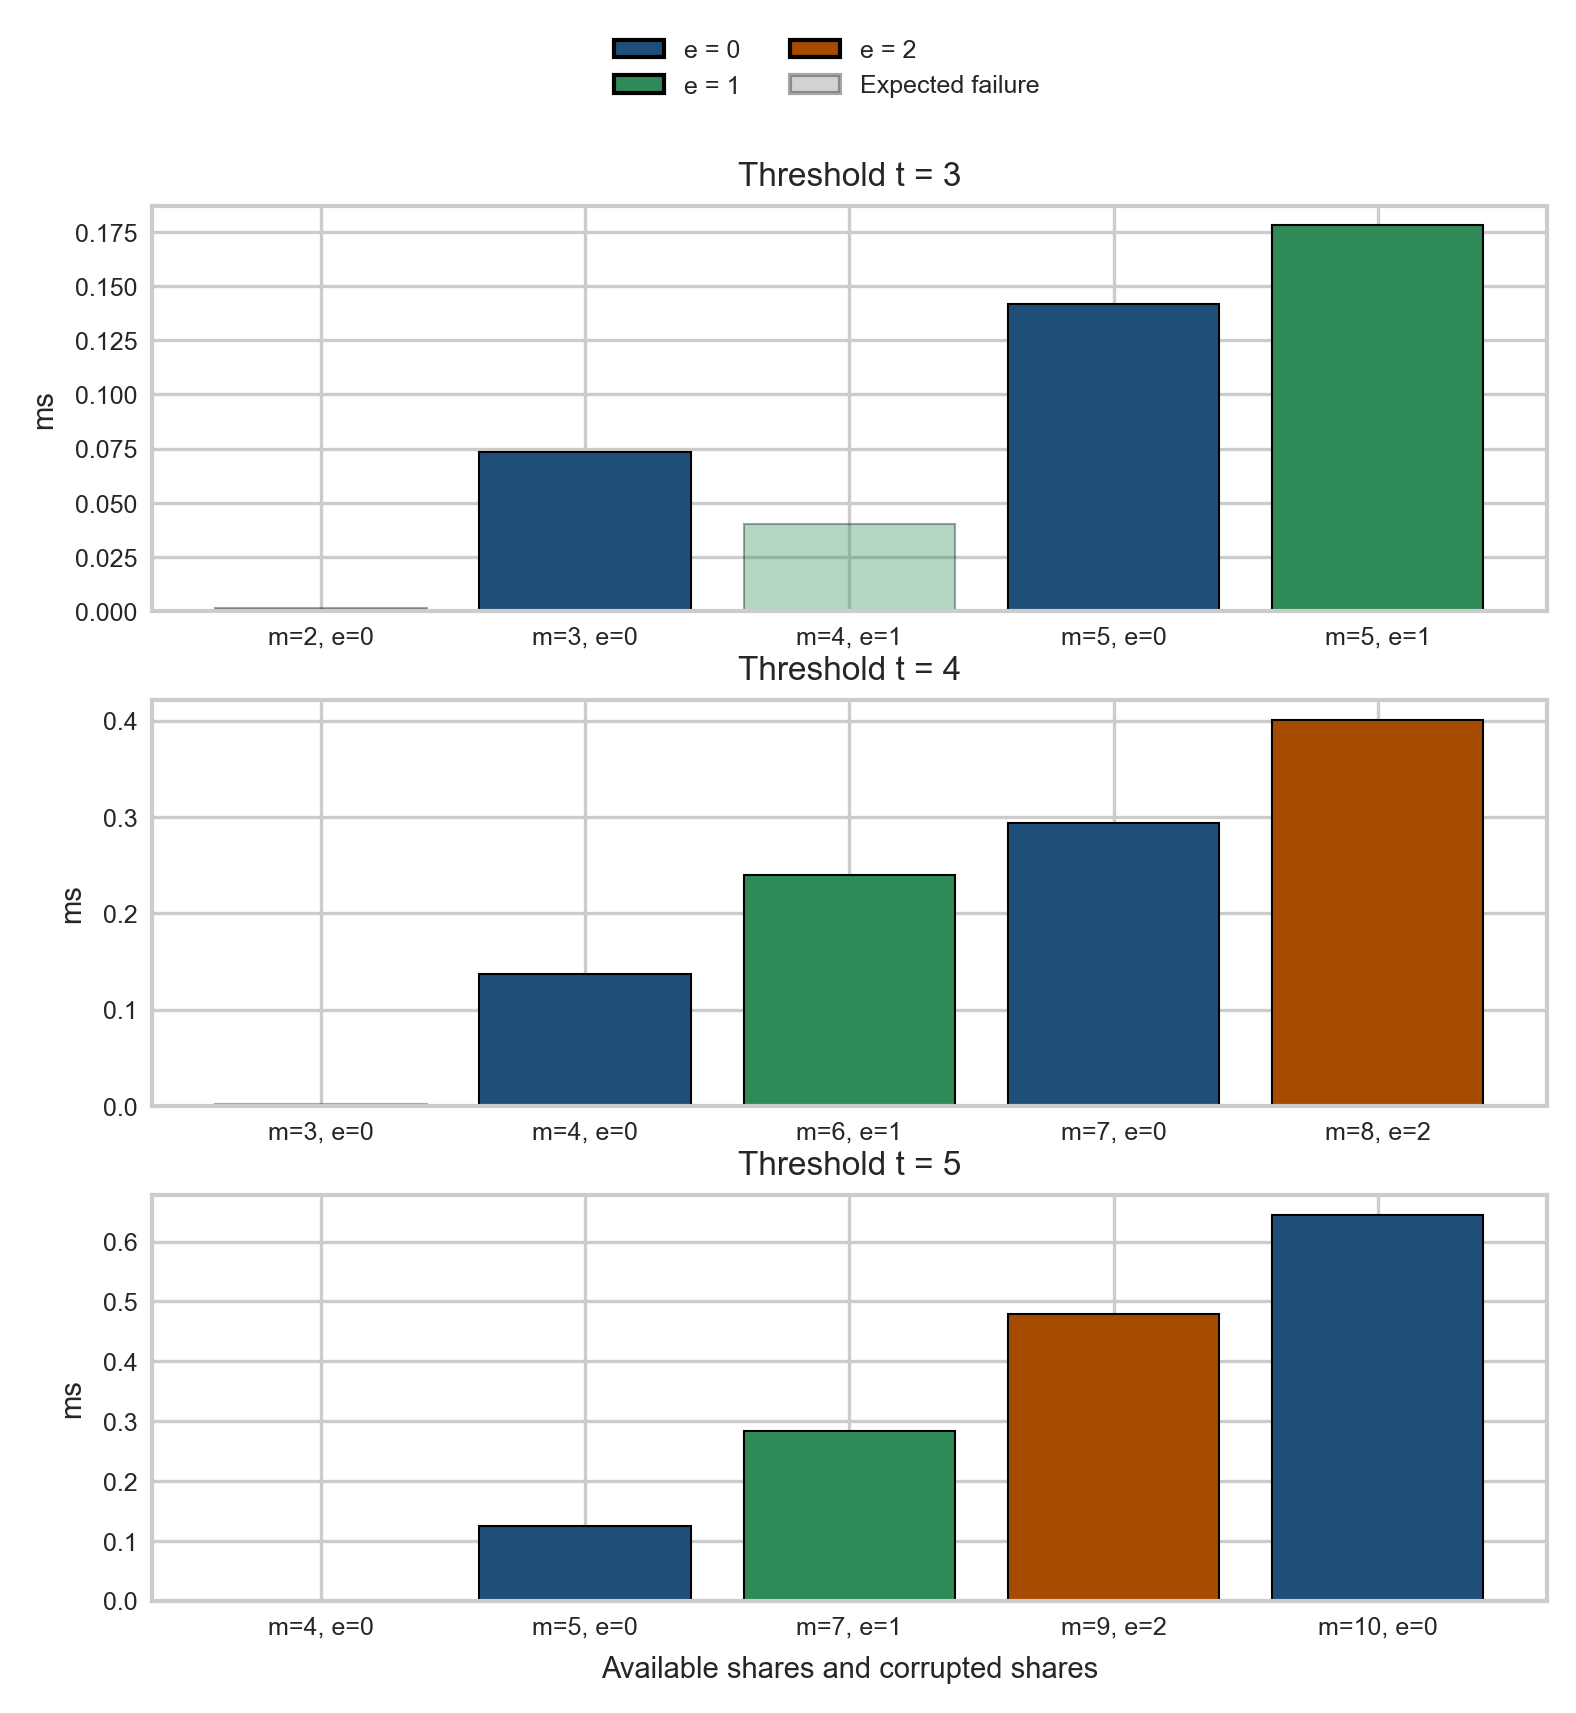
\includegraphics[width=\columnwidth,height=0.88\columnwidth,keepaspectratio]{../images/latency.png}
\caption{Mean recovery latency across threshold settings. Darker bars denote successful configurations, while faded bars denote expected failure cases.}
\label{fig:timing}
\end{figure}

\subsection{Storage Overhead}

Table~\ref{tab:storage} summarizes storage overhead under the fixed-width share format. Because each share occupies 96 bytes, overhead grows linearly with the number of generated shares. This is a predictable trade-off: the prototype gains fault tolerance and distribution flexibility at the cost of storing more total material than the original 32-byte key.

\begin{table}[H]
\caption{Storage Overhead in the Prototype}
\label{tab:storage}
\centering
\begin{tabular}{cccc}
\toprule
\textbf{$n$} & \textbf{Bytes/Share} & \textbf{Total Bytes} & \textbf{Overhead} \\
\midrule
5 & 96 & 480 & 15.0$\times$ \\
7 & 96 & 672 & 21.0$\times$ \\
8 & 96 & 768 & 24.0$\times$ \\
10 & 96 & 960 & 30.0$\times$ \\
\bottomrule
\end{tabular}
\end{table}

Although these ratios appear large compared with the original key size, the absolute storage volume remains small in practical terms. Even the largest configuration stores less than one kilobyte of share data. This is acceptable for archival key protection, password-vault backup, escrow, or multi-party administrative recovery workflows.

\subsection{Interpretation}

The results illustrate the separation between security and robustness. Increasing the threshold strengthens resistance against partial compromise but also reduces the minimum number of missing shares the system can tolerate. Adding Reed-Solomon decoding does not change that threshold policy; instead, it adds resilience against faulty inputs during reconstruction. Shamir sharing determines the access structure, whereas Reed-Solomon decoding determines the level of reconstruction fault tolerance.

Another noteworthy observation is that failure is clean. In every invalid scenario, the decoder rejected the share set rather than silently producing a usable but wrong AES key. This behavior is important because a fault-tolerant recovery system should fail closed when the algebraic constraints are unsatisfied.

The storage and timing measurements also indicate where the practical costs of the approach lie. The storage overhead is dominated by the field representation of the shares rather than by the AES key itself. The computational overhead is concentrated in the decoder, especially as the threshold and error budget grow. For the current parameter range, neither cost is prohibitive, but both would become more significant in deployments with very large thresholds or frequent reconstruction operations. This suggests that the design is best suited to backup, escrow, archival recovery, and administrative key-management settings rather than to high-frequency online use.
